\documentclass{article}
\usepackage[hyphens]{url}
\usepackage{mathtools}
\usepackage{amsmath}
\usepackage{listings}
\usepackage{graphicx}
\usepackage[margin=1in]{geometry}
\usepackage{float}
\floatstyle{boxed}
\restylefloat{figure}
\lstset{breaklines=true}
\begin{document}


\title{CS595 Intro to Web Science, Assignment \#6}
\author{Valentina Neblitt-Jones}
\date{October 31, 2013}
\maketitle



\section*{Question 1}

We know the result of the Karate Club (Zachary, 1977) split. Prove or disprove that the result of split could have been predicted by the weighted graph of social interactions. How well does the mathematical model represent reality? \\

Generously support your answer with all supporting equations, code, graphs, arguments, etc. \\

Useful sources include:  \\

\begin{itemize}
\item Original paper
	\begin{itemize}
	\item \url{http://aris.ss.uci.edu/~lin/76.pdf}
	\end{itemize}
\item Slides 
	\begin{itemize}
	\item \url{http://www-personal.umich.edu/~ladamic/courses/networks/si614w06/ppt/lecture18.ppt}
	\item \url{http://clair.si.umich.edu/si767/papers/Week03/Community/CommunityDetection.pptx}
	\end{itemize}
\item{Code and data}
	\begin{itemize}
	\item \url{http://networkx.github.io/documentation/latest/examples/graph/karate_club.html}
	\item \url{http://nbviewer.ipython.org/url/courses.cit.cornell.edu/info6010/resources/11notes.ipynb}
	\item \url{http://stackoverflow.com/questions/9471906/what-are-the-differences-between-community-detection-algorithms-in-igraph/9478989#9478989}
	\item \url{http://stackoverflow.com/questions/5822265/are-there-implementations-of-algorithms-for-community-detection-in-graphs}
	\item \url{http://konect.uni-koblenz.de/networks/ucidata-zachary}
	\item \url{http://vlado.fmf.uni-lj.si/pub/networks/data/ucinet/ucidata.htm#zachary}
	\end{itemize}
\end{itemize}
\subsection*{Answer to Question 1}


%\begin{figure}[H]
%\centering
%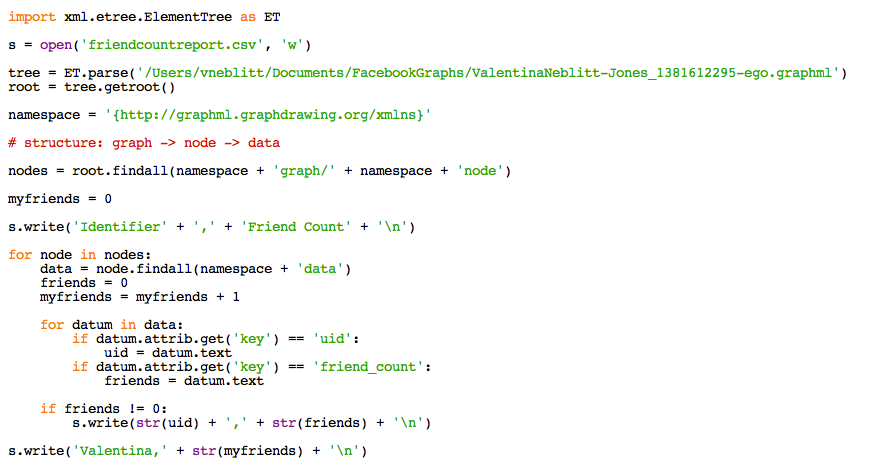
\includegraphics[scale=0.50]{q1/GetFriendCountsCode}
%\caption{Showing Friend Count}
%\label{GetFriendCountsCode}
%\end{figure}

\begin{table}[!h]
\centering

\begin{tabular}{c c c c}
\hline
Identifier & Model &  Actual & Hit/Miss \\
\hline
\hline
1 & Mr. Hi & Mr. Hi & Hit \\
2 & Mr. Hi & Mr. Hi & Hit \\
3 & Mr. Hi & Mr. Hi & Hit \\
4 & Mr. Hi & Mr. Hi & Hit \\
5 & Mr. Hi & Mr. Hi & Hit \\
6 & Mr. Hi & Mr. Hi & Hit \\
7 & Mr. Hi & Mr. Hi & Hit \\
8 & Mr. Hi & Mr. Hi & Hit \\
9 & Mr. Hi & Mr. Hi & Hit \\
10 & Mr. Hi & John & Miss \\
11 & Mr. Hi & Mr. Hi & Hit \\
12 & Mr. Hi & Mr. Hi & Hit \\
13 & Mr. Hi & Mr. Hi & Hit \\
14 & Mr. Hi & Mr. Hi & Hit \\
15 & John & John & Hit \\
16 & John & John & Hit \\
17 & Mr. Hi & Mr. Hi & Hit \\
18 & Mr. Hi & Mr. Hi & Hit \\
19 & John & John & Hit \\
20 & Mr. Hi & Mr. Hi & Hit \\
21 & John & John & Hit \\
22 & Mr. Hi & Mr. Hi & Hit \\
23 & John & John & Hit \\
24 & John & John & Hit \\
25 & John & John & Hit \\
26 & John & John & Hit \\
27 & John & John & Hit \\
28 & John & John & Hit \\
29 & John & John & Hit \\
30 & John & John & Hit \\
31 & John & John & Hit \\
32 & Mr. Hi & John & Miss \\
33 & John & John & Hit \\
34 & John & John & Hit \\
\hline
\end{tabular}
\caption{Results of Model vs. Actual}
\end{table}

32 hits, 2 misses \\
94\% hits, 6\% misses \\

\newpage

\section*{Extra Credit, 3 Points}

We know the group split into two different groups. Suppose the disagreements in the group were more nuanced -- what would the clubs look like if they split into groups of 3, 4, and 5?

%\begin{table}[!h]
%\centering
%\caption{Results of Model vs. Actual}
%\begin{tabular}{c c c c}
%\hline
%Identifier & Model &  Actual & Hit/Miss \\
%\hline
%\hline
%0.150 & 0.014 & Mr. Hi & Hit \\
%0.085 & John & Mr. Hi & Hit \\
%\hline
%\end{tabular}
%\end{table}

\subsection*{Answer to Extra Credit}





\newpage

\section*{Resources}

\begin{itemize}
\item Csardi, Gabor. Network Analysis with igraph. \url{http://igraph.sourceforge.net/igraphbook/index.html}
\item Poulson, Barton. R Statistics Essential Training. \url{http://www.lynda.com/course20/R-tutorials/R-Statistics-Essential-Training/142447-2.html}
\item Rice, Ken \& Lumley Thomas. Writing Loops. \url{http://faculty.washington.edu/kenrice/sisg/SISG-08-05.pdf}
\item Sourceforge.net. Network Analysis and Visualization. \url{http://igraph.sourceforge.net/doc/R/00Index.html}
\item Stack Overflow. Are there implentations of algorithms for community detection in graphs? \url{http://stackoverflow.com/questions/5822265/are-there-implementations-of-algorithms-for-community-detection-in-graphs}
\item Stack Overflow. What are the differences between community detection algorithms in igraph? \url{http://stackoverflow.com/questions/9471906/what-are-the-differences-between-community-detection-algorithms-in-igraph/9478989#9478989}
\item Zachary, Wayne. An Information Flow Model for Conflict and Fission in Small Groups. \url{http://aris.ss.uci.edu/~lin/76.pdf}


\end{itemize}

\end{document}